\subsection{Dreamfusion}\label{dreamfusion}

DreamFusion, as introduced by \citeauthor{pooleDreamfusion}, marks a significant advancement in the field of 3D modeling. Utilizing Neural Radiance Fields (NeRF), DreamFusion employs a novel technique known as Score Distillation Sampling (SDS) to generate coherent 3D objects and scenes from a variety of text prompts. This approach diverges from traditional methods that depend on pre-existing images from multiple angles, as DreamFusion dynamically generates these images during training using a 2D diffusion model.

Central to DreamFusion is the use of Differentiable Image Parameterization (DIP), as described by \citep{mordvintsevDIP}. This technique enables the generation of images \( x \) through parameters \( \theta \) and a differentiable generator \( g \), offering refined optimization capabilities even at the pixel level \citep{pooleDreamfusion}. This marks a shift from the conventional approach of diffusion models, which usually produce outputs similar to their training data. In DreamFusion, the parameters \( \theta \) define 3D volumes, with \( g \) functioning as a volumetric renderer. 

This method offers an innovative approach to transforming text into 3D models, as depicted in Figure~\ref{fig:figureDreamfusion}. This process employs several key components: a text prompt with the desired goal that serves as a guide, Google's Imagen as the text-to-image diffusion model \citep{saharia2022imagen}, an imporved version of Neural Radiance Field, the mip-NeRF 360 \citep{barron2022mipnerf} ``that reduces aliasing'' \citep{pooleDreamfusion}, and the Score Distillation Sampling (SDS) for the loss function.

\begin{figure}[ht]
  \centering
    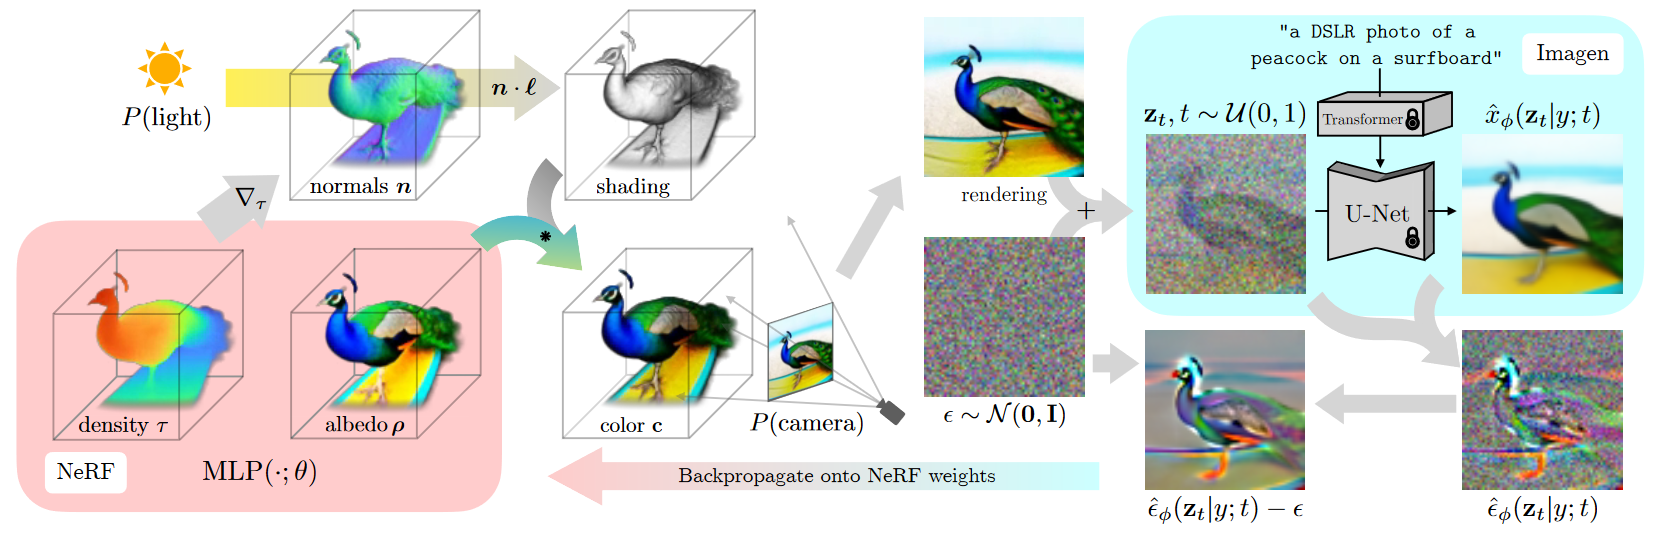
\includegraphics[width=1\columnwidth]{figures/Dreamfusion.png}
    \caption{Overview of DreamFusion's process for transforming text into 3D models, illustrating the integration of Neural Radiance Fields, Score Distillation Sampling, and diffusion models. Image adapted from \citep{pooleDreamfusion}.}\label{fig:figureDreamfusion}
\end{figure}

At the center of the rendering process is the Neural Radiation Field, which is represented as \( \text{MLP}(\cdot; \theta) \), where the dot \(\cdot\) denotes the input of 3D coordinates and viewing directions. This input is important to determine how light and color interact in 3D space.~\(\theta\) symbolizes the parameters of the MLP that are fine-tuned during training. These parameters determine how the MLP interprets its input (the 3D coordinates and viewing directions) to produce the final output, such as the color and density at each point in the 3D model.

The process of generating 3D scenes in DreamFusion begins with the random initialization of the NeRF MLP's parameters. This is followed by the selection of random camera angles and lighting positions, ensuring realistic and varied perspectives \citep{pooleDreamfusion}. Multiplying the light position \( l \) by the normals derived directly from the density gradients calculated during NeRF training produces the shading output, an essential element for realism. Additionally, the inherent color of objects, or albedo, is also generated during the NeRF rendering phase. By combining albedo and shading effects, the NeRF can render accurate colors for every point in the scene, resulting in detailed visual representations from any chosen viewing angle. Following these steps, an image is sampled from the current state of the NeRF representation.

Unlike traditional NeRFs, which rely on the loss of total squared error for training, DreamFusion uses Score Distillation Sampling (SDS) to refine the model. SDS differs from the total squared error approach in that the pixel values are not compared directly. Instead, the model initially adds random noise \(\epsilon\) to its rendering, simulating a `diffusion' process \citep{pooleDreamfusion}. It then uses the Imagen diffusion model to evaluate the diffused rendering based on its knowledge of what makes a high quality image based on the given text prompt. Considering the current time step \(t\), Imagenl aims to predict the less noisy version of the image \(x\) of the previous timestep. The predicted noise \( \hat{\epsilon}_\phi(z_t | y; t) \) is calculated based on the current state of the image \(z_t\), the guiding text prompt \(y\) and the specific time step \(t\). This introduction of noise is used to iteratively guide the rendering closer to an image that matches the text description.

The next step involves subtracting the predicted noise from the diffused image, resulting in a low variance update direction \citep{pooleDreamfusion}. Essentially, this is a clearer direction of how the NeRF should change to produce an image that better matches the text prompt. This update direction is then backpropagated to the NeRF MLP, which allows its parameters \(\theta\) to be fine-tuned accordingly.

The primary SDS function, as formualted by \citeauthor{pooleDreamfusion}, is denoted as:~\[
\nabla_{\theta}\mathcal{L}_{\text{SDS}}(\phi,\mathbf{x}=g(\theta))\triangleq\mathbb{E}_{t,\epsilon}\left[w(t)\left(\hat{\epsilon}_{\phi}({\mathbf{z}}_{t};y,t)-\epsilon\right){\frac{\partial\mathbf{x}}{\partial\theta}}\right]
\] In this equation, \( w(t) \) acts as a weighting factor, modifying the influence of different components within the formula. Additionally, the term \( \frac{\partial\mathbf{x}}{\partial\theta} \) indicates how changes in the model's parameters \( \theta \) affect the image \( \mathbf{x} \), guiding the optimization process.

Despite DreamFusion's promising results, it is not without limitations. The model tends to exhibit a lower level of detail, partly due to its reliance on a \( 64 \times 64 \) image model \citep{lin2023magic3d}. Furthermore, while SDS is an effective loss function, it sometimes leads to ``oversaturated and oversmoothed results \([\ldots]\)'' \citep{pooleDreamfusion}. Another aspect to consider with SDS is the mode-seeking behavior, which potentially limits the variety of results generated. This limitation is strengthened by the use of KL divergence, ``which has been previously noted to have mode-seeking properties in the context of variational inference and probability density distilaltion''\citep{pooleDreamfusion}. This tendency of the model to prioritize the most frequent patterns can lead to a trade-off between accuracy and diversity, so ``it may be unclear if minimizing this loss will produce good samples'' \citep{pooleDreamfusion}. This statement highlights a major challenge in machine learning, especially with generative models such as DreamFusion. Minimizing loss, a standard method for improving model performance, does not always lead to high-quality or diverse results. There is a risk of overfitting, where the model can reproduce the training data very well, but is less able to generate new and diverse results.